\section{利率和现值分析}
\begin{enumerate}[label=\arabic{section}.\arabic*]
    \item \sol
    \begin{enumerate}[label=\alph*)]
        \item $r_{\eff a}=(1+0.1/2)^2-1=10.25\%$.
        \item $r_{\eff b}=(1+0.1/4)^4-1 \approx 10.38\%$.
        \item $r_{\eff c}=\e^{0.1}-1 \approx 10.52\%$.
    \end{enumerate}
    \item \sol\\
    设需要$n$年钱变为两倍,则
    \[\e^{0.1n}=2 \Rightarrow n=\frac{\ln 2}{0.1} \approx 6.93.\]
    \item \sol\\
    设需要$n$年钱变为四倍,则
    \begin{align*}
        (1+0.05)^n=4& \Rightarrow n \approx 28.41,\\
        (1+0.04)^n=4& \Rightarrow n \approx 35.35.
    \end{align*}
    \item \sol\\
    设需要$n$年钱变为三倍,则
    \[\e^{nr}\approx(1+r)^n=3 \Rightarrow n \approx \frac{\ln 3}{r}.\]
    \item \sol {\kaishu \textcolor{blue}{注意:每月支付说明有60次投资.}}\\
    设需要投资$x$元,则
    \[x\sum_{i=1}^{60}(1+0.06/12)^i=\frac{1.005x(1-1.005^{60})}{1-1.005}=100000 \Rightarrow n \approx 1426.15.\]
    \item \sol\\
    计算现值:
    \[-1000+\frac{-1200}{1.06}+\frac{800}{1.06^2}+\frac{900}{1.06^3}+\frac{800}{1.06^4}=-30.75<0,\]
    所以这不是一个值得的投资.
    \item \sol\\
    记这两个现金流的现值分别为$S_1,S_2$,则
    \begin{align*}
        S_1 & = \frac{20}{1+r}+\frac{20}{(1+r)^2}+\frac{20}{(1+r)^3}+\frac{15}{(1+r)^4}+\frac{10}{(1+r)^5}+\frac{5}{(1+r)^6},\\
        S_2 & = \frac{10}{1+r}+\frac{10}{(1+r)^2}+\frac{15}{(1+r)^3}+\frac{20}{(1+r)^4}+\frac{20}{(1+r)^5}+\frac{20}{(1+r)^6}.
    \end{align*}
    \begin{enumerate}[label=\alph*)]
        \item $r=0.03,S_1=82.71, S_2 = 84.63$,第二个现金流更可取.
        \item $r=0.05,S_1=78.37, S_2 = 78.60$,第二个现金流更可取.
        \item $r=0.10,S_1=69.01, S_2 = 65.99$,第一个现金流更可取.
    \end{enumerate}
    \item \sol\\
    记现值为$S$,则\[S=-10000+\sum_{i=1}^{10}\frac{500}{(1+r/2)^i}+\frac{10000}{(1+r/2)^{10}},\]
    \begin{enumerate}[label=\alph*)]
        \item $r = 0.06, S = 1706.04$.
        \item $r = 0.10, S = 0$.
        \item $r = 0.12, S = -736.01$.
    \end{enumerate}
    \item \sol\\
    记有效利率为$r$,则
    \[4200-1000=160\sum_{i=1}^{24}\frac{1}{(1+r)^i} \Rightarrow \frac{1-\left(\frac{1}{1+r}\right)^{24}}{4}=20 \Rightarrow r=0.15.\]
    \item \sol\\
    第一个现金流序列的现值为
    \[22+\frac{7}{1.2}+\frac{8}{1.2^2}+\frac{9}{1.2^3}+\frac{10}{1.2^4}-\frac{4}{1.2^5}=41.812,\]
    第二个现金流序列的现值为
    \[9+\frac{24}{1.2}+\frac{7}{1.2^2}+\frac{8}{1.2^3}+\frac{9}{1.2^4}-\frac{8}{1.2^5}=39.616,\]
    第三个现金流序列的现值为
    \[9+\frac{11}{1.2}+\frac{26}{1.2^2}+\frac{7}{1.2^3}+\frac{8}{1.2^4}-\frac{12}{1.2^5}=39.309,\]
    第四个现金流序列的现值为
    \[9+\frac{11}{1.2}+\frac{13}{1.2^2}+\frac{28}{1.2^3}+\frac{7}{1.2^4}-\frac{16}{1.2^5}=40.344,\]
    因此,公司应在一年后购买新机器.
    \item \sol\\
    这家公司可以在第1、2、3、4年的年初购买新机器,其对应的六年现金流如下(以1000美元为单位):
    \begin{itemize}
        \item 在第一年的年初购买新机器:22,7,8,9,10,$-4$
        \item 在第二年的年初购买新机器:9,25,7,8,9,$-9$
        \item 在第三年的年初购买新机器:9,11,28,7,8,$-14$
        \item 在第四年的年初购买新机器:9,11,13,31,7,$-19$
    \end{itemize}
    对于年利率$r=0.10$,第一个现金流序列的现值为
    \[22+\frac{7}{1.1}+\frac{8}{1.1^2}+\frac{9}{1.1^3}+\frac{10}{1.1^4}-\frac{4}{1.1^5}=46.08,\]
    其他现金流的现值可用同样的方法计算出. 这四个现金流的现值分别是
    \[46.08, 44.08, 44.17, 46.02,\]
    因此,公司应在一年后购买新机器.
    \item \sol\\
    由于银行收取两个百分点的费用,这个贷款的实际费用为$120000 \times 0.98=117600$. 每月需要支付利息$120000 \times 0.5\%=600$. 所以该贷款的现金流为
    \begin{table}[H]
        \centering
        \begin{tabular}{c|c|c|c|c|c|c}
            时间 & 0 & 1 & 2 & $\cdots$ & 35 & 36 \\ \hline
            现金流 & 117600 & $-600$ & $-600$ & $\cdots$ & $-600$ & $-120600$
        \end{tabular}
    \end{table}
    记有效利率为$r$,则
    \[117600=600\sum_{i=1}^{35}\frac{600}{(1+r)^i}+\frac{120600}{(1+r)^{36}} \Rightarrow r \approx 0.5615\%.\]
    \item \sol\\
    第一种还款方式的现值为16000美元,第二种还款方式的现值为
    \[S=10000+10000\e^{-10r},\]
    \begin{enumerate}[label=\alph*)]
        \item $r = 0.02, S = 18187.31$,第一种还款方式更可取.
        \item $r = 0.05, S = 16065.31$,第一种还款方式更可取.
        \item $r = 0.10, S = 13678.79$,第二种还款方式更可取.
    \end{enumerate}
    \item \sol\\
    现金流为
    \begin{table}[H]
        \centering
        \begin{tabular}{c|c|c|c|c|c|c}
            时间 & 0 & 0.5 & 1 & $\cdots$ & 4.5 & 5 \\ \hline
            现金流 & $-1000$ & 30 & 30 & $\cdots$ & 30 & 1030
        \end{tabular}
    \end{table}
    现值为
    \[-1000+\sum_{i=1}^{9}\frac{30}{\e^{0.05i/2}}+\frac{1030}{\e^{0.05\times 5}}=40.94.\]
    \item \sol\\
    $\displaystyle \left(1+\frac{0.05}{n}\right)^n$表示一年后的存款金额,如果最初存入1,名义利率为5\%,一年内复利$n$次,复合次数越多,存款金额越多.
    \item \sol\\
    $n$天后可得到的利息为
    \[A=100(\e^{0.06n/365}-1),\]
    \begin{enumerate}[label=\alph*)]
        \item $n = 30, A = 0.49$.
        \item $n = 60, A = 0.99$.
        \item $n = 120, A = 1.99$.
    \end{enumerate}
    \item \sol\\
    $1000\e^{3r}+2000\e^{2r}+3000\e^{r}$.
    \item \sol \[\frac{3}{1.05}+\frac{5}{1.05^2}-\frac{6}{1.05^3}+\frac{5}{1.05^4}=6.74.\]
    \item \sol \[20+\frac{10}{1+r}>0+\frac{34}{1+r} \Rightarrow r>0.2.\]
    \item \sol \[1500=1000\e^{0.6t} \Rightarrow t=6.7578.\]
    \item \sol \[A\e^{-rs}+\sum_{n=1}^{\infty} A\e^{-r(s+nt)}=A\e^{-rs}\sum_{n=0}^{\infty} \e^{-nrt}=\frac{A\e^{-rs}}{1-\e^{-rt}}.\]
    \item \pro
    \begin{enumerate}[label=\alph*)]
        \item 因为$D(t)=D\e^{rt}$,当$r>0, h \to 0$时,$\e^{rh} \sim rh+1$,所以
        \[D(t+h)=D\e^{r(t+h)}=D\e^{rt}\e^{rh} = D(t)\e^{rh} \approx D(t)(1+rh)=D(t)+rhD(t).\]
        \item 由上一小问,得
        \[\frac{D(t+h)-D(t)}{h} \approx rD(t) \Rightarrow \lim_{h \to 0}\frac{D(t+h)-D(t)}{h} = \lim_{h \to 0}rD(t) \Rightarrow D'(t)=rD(t).\]
        \item 由上一小问,得
        \[\begin{cases}
            \displaystyle\frac{D'(t)}{D(t)}=r,\\D(0)=D,
        \end{cases} \Rightarrow \ln D(t)=rt+\ln D \Rightarrow D(t)=D\e^{rt}.\]
    \end{enumerate}
    \item \sol\\
    利用命题4.2.1,令两个现金流分别为$B_n,C_n$,有$B_n \geq C_n, \displaystyle \sum_{i=1}^k B_i \geq \sum_{i=1}^k C_i(k=1,2,3)$,所以前一个现金流更可取.
    \item \sol
    \begin{enumerate}[label=\alph*)]
        \item $100(1+r)^2=110 \Rightarrow r=0.0488$.
        \item 有$r=\begin{cases}
            \sqrt{1.2}-1, & p=0.5 \\ 0, & p=0.5
        \end{cases}$,所以$\displaystyle E(r)=\frac{\sqrt{1.2}-1}{2}=0.0477$.
    \end{enumerate}
    \item \sol \[\frac{1000}{\e^{0.08\times 10}}=449.33.\]
    \item \sol \begin{align*}
        100 & = \frac{40}{1+r}+\frac{70}{(1+r)^2} \Rightarrow r=0.0602,\\
        100 & = \frac{70}{1+r}+\frac{40}{(1+r)^2} \Rightarrow r=0.0728.
    \end{align*}
    \item \sol {\kaishu \textcolor{blue}{注意:b)问由于翻译原因,所问不是投资回报率是否等于11\%,而是是否大于11\%.}}
    \begin{enumerate}[label=\alph*)]
        \item 不需要,每个周期的回报率超过10\%当且仅当$\displaystyle \sum_{i=1}^n \frac{x_i}{1.1^i}>1$.
        \item 是,因为$\displaystyle \frac{8}{1.11}+\frac{16}{1.11^2}+\frac{110}{1.11^3}=100.624>100$.
    \end{enumerate}
    \item \sol\\
    由于$X_1,X_2 \sim N(60,25)$,所以$\displaystyle 1.1X_1+X_2\sim N(126,55.25)$,则
    \[P\left(\frac{X_1}{1.1}+\frac{X_2}{1.1^2}>100\right)=P(1.1X_1+X_2>121)=P\left(Z>\frac{121-126}{\sqrt{55.25}}\right)=\Phi(0.6727)=0.7494.\]
    \item \sol \[r_a=\frac{1+r}{1+r_i}-1=\frac{1.05}{1.03}-1=1.942\%.\]
    \item \pro
    \begin{enumerate}[label=\alph*)]
        \item 由于$\displaystyle \lim_{r \to +\infty}P(r)=c_0<0,\lim_{r \to -1}P(r)=+\infty$,所以在$r>-1$上必有解,可证得该解唯一.
        \item 取$n=3,c_0=-1,c_1=-3,c_2=1$,则$\displaystyle P(-0.8)=9,P(0)=-3,P(1)=-\frac{9}{4}$,显然此时$P(r)$不单调.
    \end{enumerate}
    \item \sol \[\mathrm{PV}(a)=-\frac{1000}{1.08}+\frac{900}{1.05^2}+\frac{800}{1.05^3}-\frac{1200}{1.08^4}+\frac{700}{1.05^5}=247.90>0,\]所以应该投资.
    \item \pro
    \[\frac{\d \bar{r}(t)}{\d t}=\frac{tr(t)-\int_0^t r(s)\,\d s}{t^2},\]
    因为$\displaystyle \int_0^t r(s)\,\d s \leq \int_0^t r(t)\,\d s=tr(t)$,则
    \[tr(t)-\int_0^t r(s)\,\d s \geq 0 \Rightarrow \frac{\d \bar{r}(t)}{\d t} \geq 0,\]
    所以$\bar{r}(t)$也是$t$的非减函数.
    \item \pro\\
    有\[P(\alpha t)=\exp\left[-\int_0^{\alpha t}r(s)\,\d s\right]=\exp\left[\alpha t \bar{r}(\alpha t)\right],P^{\alpha}(t)=\exp[-\alpha t\bar{r}(t)],\]
    所以\[P(\alpha t) \geq [P(t)]^{\alpha} \iff \bar{r}(\alpha t) \leq \bar{r}(t) \iff \bar{r}(t)\text{是}t\text{的非减函数}.\]
    \item \pro
    \begin{enumerate}[label=\alph*)]
        \item \[P(t)=\mathrm{exp}\left(-\int_0^t r(s)\,\mathrm{d} s\right),P'(t)=-r(t)\mathrm{exp}\left(-\int_0^t r(s)\,\mathrm{d} s\right),r(t)=-\frac{P'(t)}{P(t)}.\]
        \item \[P(t)=\mathrm{exp}\left(-\int_0^t r(s)\,\mathrm{d} s\right),\ln P(t)=-\int_0^t r(s)\,\mathrm{d} s,\bar{r}(t)=-\frac{\ln P(t)}{t}.\]
    \end{enumerate}
    \item \sol
    \begin{figure}[H]
        \centering
        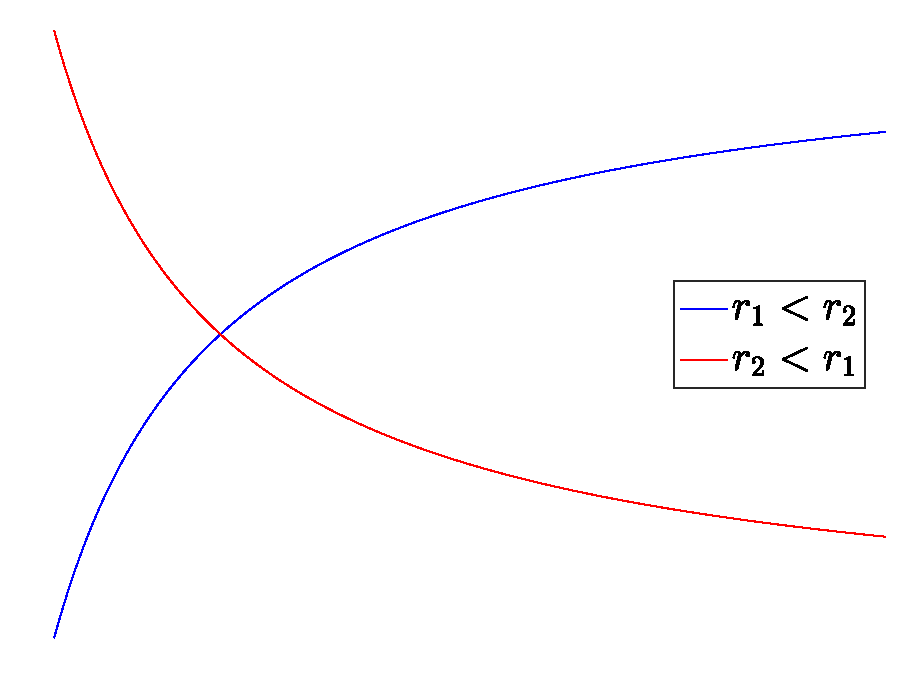
\includegraphics[scale=0.5]{4.35.eps}
    \end{figure}
\end{enumerate}
\clearpage